%%%%%%%%%%%%%%%%%%%%%%%%%%%%%%%%%%%%%
%                                   %
% Compile with XeLaTeX and biber    %
%                                   %
% Questions or comments:            %
%                                   %
% joshua dot mcneill at uga dot edu %
%                                   %
%%%%%%%%%%%%%%%%%%%%%%%%%%%%%%%%%%%%%

\documentclass{beamer}
  % Read in standard preamble (cosmetic stuff)
  %%%%%%%%%%%%%%%%%%%%%%%%%%%%%%%%%%%%%%%%%%%%%%%%%%%%%%%%%%%%%%%%
% This is a standard preamble used in for all slide documents. %
% It basically contains cosmetic settings.                     %
%                                                              %
% Joshua McNeill                                               %
% joshua dot mcneill at uga dot edu                            %
%%%%%%%%%%%%%%%%%%%%%%%%%%%%%%%%%%%%%%%%%%%%%%%%%%%%%%%%%%%%%%%%

% Beamer settings
% \usetheme{Berkeley}
\usetheme{CambridgeUS}
% \usecolortheme{dove}
% \usecolortheme{rose}
\usecolortheme{seagull}
\usefonttheme{professionalfonts}
\usefonttheme{serif}
\setbeamertemplate{bibliography item}{}

% Packages and settings
\usepackage{fontspec}
  \setmainfont{Charis SIL}
\usepackage{hyperref}
  \hypersetup{colorlinks=true,
              allcolors=blue}
\usepackage{graphicx}
  \graphicspath{{../../figures/}}
\usepackage[normalem]{ulem}
\usepackage{enumerate}

% Document information
\author{M. McNeill}
\title[FREN2001]{Français 2001}
\institute{\url{joshua.mcneill@uga.edu}}
\date{}

%% Custom commands
% Lexical items
\newcommand{\lexi}[1]{\textit{#1}}
% Gloss
\newcommand{\gloss}[1]{`#1'}
\newcommand{\tinygloss}[1]{{\tiny`#1'}}
% Orthographic representations
\newcommand{\orth}[1]{$\langle$#1$\rangle$}
% Utterances (pragmatics)
\newcommand{\uttr}[1]{`#1'}
% Sentences (pragmatics)
\newcommand{\sent}[1]{\textit{#1}}
% Base dir for definitions
\newcommand{\defs}{../definitions}


  % Packages and settings

  % Document information
  \subtitle[Oui ou non]{Les questions oui ou non}

\begin{document}
  % Read in the standard intro slides (title page and table of contents)
  \begin{frame}
    \titlepage
    \tiny{Office: % Basically a variable for office hours location
Gilbert 121\\
          Office hours: % Basically a variable for office hours
 lundi, mercredi, vendredi 10:10--11:10
}
  \end{frame}

  \begin{frame}{Annonces}
    \begin{itemize}
      \item Rendez le devoir 1 lundi.
      \item[] \gloss{Turn in homework 1 Monday.}
    \end{itemize}
  \end{frame}

  \begin{frame}{}
    \begin{center}
      \Large Quiz
    \end{center}
  \end{frame}

  \begin{frame}{Questions au sujet de la famille}
    \begin{columns}[T]
      \column{0.5\textwidth}
        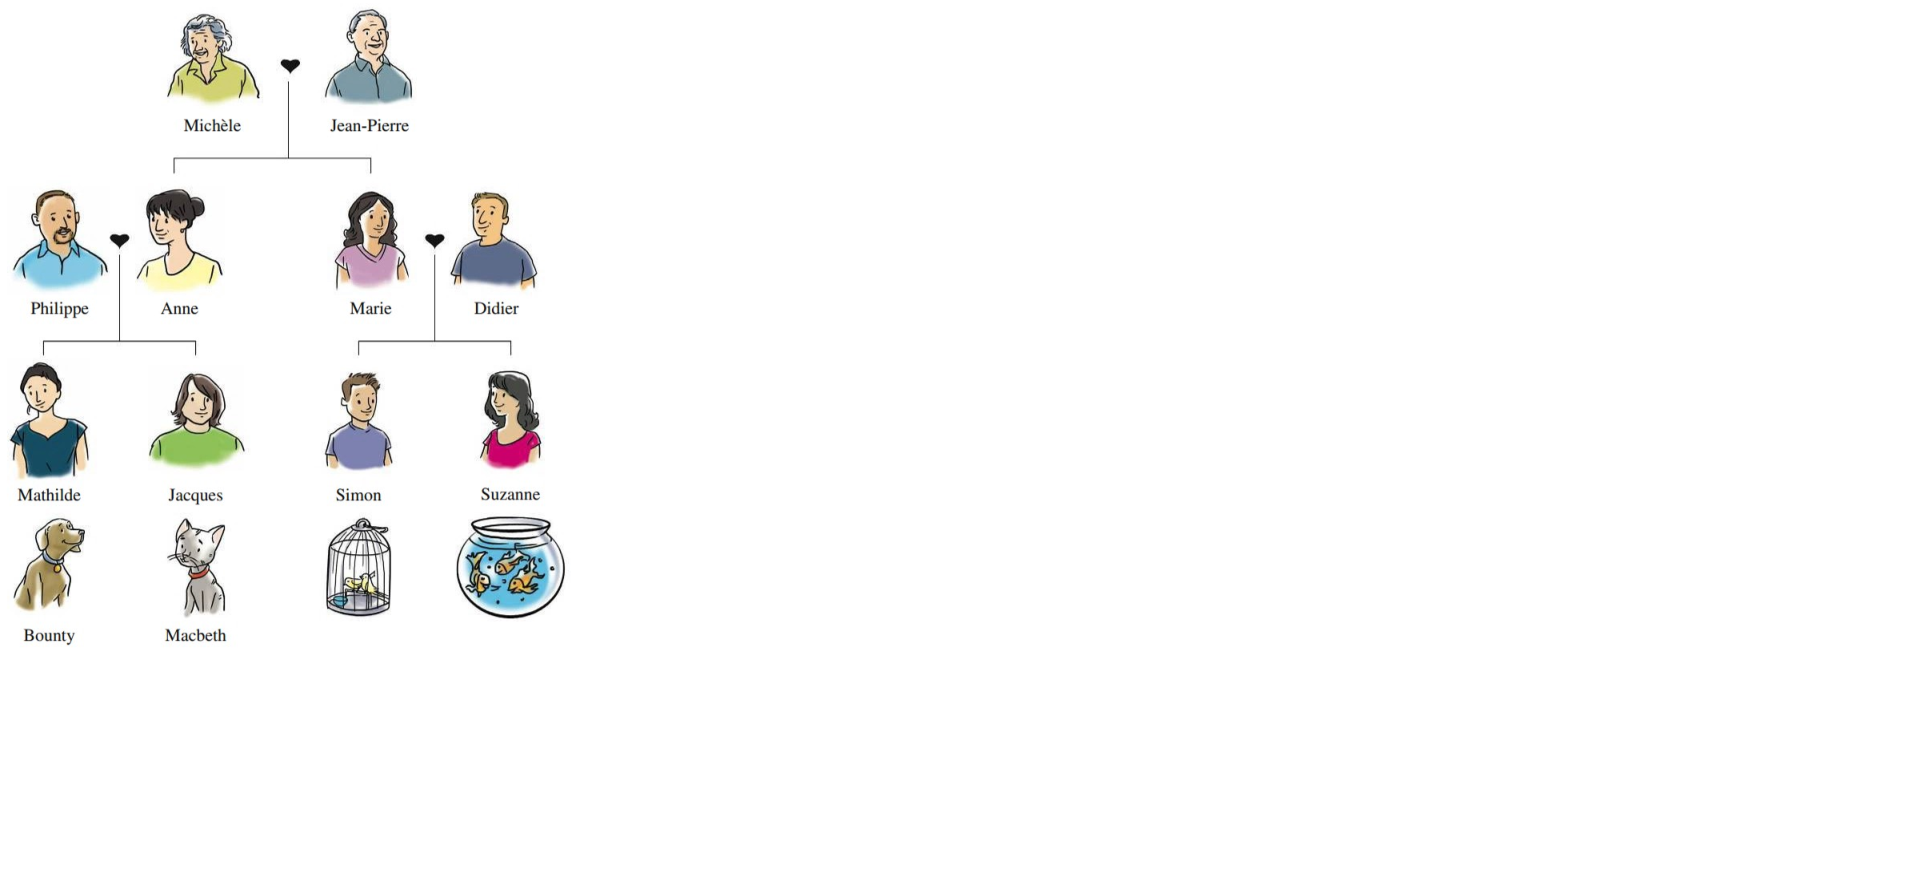
\includegraphics[scale=0.4]{famille_de_jacques.png}
      \column{0.5\textwidth}
        {\scriptsize
          \lexi{oui}, \lexi{non} ou \lexi{si}?
          \begin{enumerate}
            \item Est-ce que la mère de Jacques s'appelle Anne?
            \item Est-ce que Jacques a une sœur?
            \item Est-ce que sa sœur s'appelle Mathilde?
            \item Est-ce qu'il a trois cousins?
            \item Est-ce que ses grands-parents s'appellent Jean-Pierre et Michèle?
            \item Il n'a pas de chiens?
            \item Est-ce que sa tante est divorcée?
            \item Est-ce qu'elle a deux enfants?
            \item Est-ce que la cousine de Jacques s'appelle Suzanne?
            \item Suzanne n'a pas de frères?
            \item Le mari de Marie s'appelle Philippe?
          \end{enumerate}
        }
    \end{columns}
  \end{frame}

  \begin{frame}{Entrevue}
    \gloss{Use the following prompts to form questions to ask a partner.
    For example:} \\
    \begin{description}
      \item[] \emph{avoir des frères}
      \item[E1:] Est-ce que tu as des frères?
      \item[E2:] Je n'ai pas de frère.
    \end{description}
    \begin{columns}
      \column{0.5\textwidth}
        \begin{enumerate}
          \item travailler beaucoup
          \item jouer du piano ou de la guitare
          \item jouer au football ou au tennis
          \item regarder la télé
        \end{enumerate}
      \column{0.5\textwidth}
        \begin{enumerate}
          \setcounter{enumi}{4}
          \item regarder des films
          \item préparer le dîner
          \item inviter des copains à dîner
        \end{enumerate}
    \end{columns}
  \end{frame}

  \begin{frame}{Pictionary}
    \gloss{In groups of 4, take turns drawing pictures representing vocabulary items.
    Whoever is not drawing in the group should try to guess what it is.
    Whoever guesses first gets a point.
    Try to get the most points.
    \alert{The \lexi{dessinateur/dessinatrice} \gloss{drawer} can and should respond with \lexi{oui} or \lexi{non} followed by a complete sentence.}
    For example:}
    \begin{columns}
      \column{0.6\textwidth}
        \begin{description}
          \item[] (A picture of a marker is drawn by E1.)
          \item[E2:] C'est un stylo.
          \item[E1:] Non, ce n'est pas un stylo.
          \item[E3:] C'est un feutre.
          \item[E1:] Oui, c'est un feutre.
        \end{description}
      \column{0.4\textwidth}
        \begin{center}
          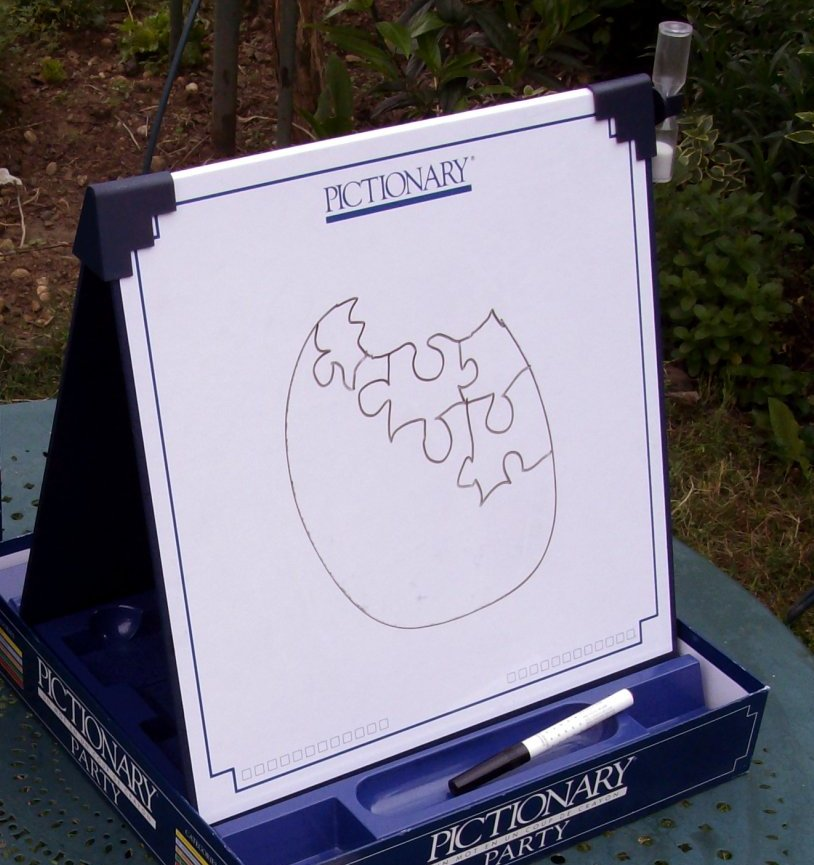
\includegraphics[scale=0.4]{pictionary.jpg}
        \end{center}
    \end{columns}
  \end{frame}

  \begin{frame}{}
    \begin{center}
      \Large Questions?
    \end{center}
  \end{frame}
\end{document}
